%% \chapter{Properties and flavours \Author{P. Brisk}\\\progressbar[0.4\textwidth]{writing}{80}}
\chapter{Properties and flavours \Author{P. Brisk}}
\inputprogress
\label{chap:properties_and_flavours}
\graphicspath{{Figs/}{properties_and_flavours/Figs/}{part1/properties_and_flavours/Figs/}{tikz/}{properties_and_flavours/tikz/}{part1/properties_and_flavours/tikz/}}
\inputpath{{tikz/}{properties_and_flavours/tikz/}{part1/properties_and_flavours/tikz/}}


\section{Preliminaries}

Recall from the previous chapter that a procedure is in SSA form if
every variable is defined once, and every use of a variable corresponds
to exactly one definition. Many variations, or flavors, of SSA form that 
satisfy these criteria can be defined, each offering its own considerations.
For example, different flavors vary in terms of the number of $\phi$-functions,
which affects the size of the intermediate representation; some are more difficult to construct, maintain, and destruct
compared to others. This chapter explores these SSA flavors and provides
insight onto the contexts that favor some over others. 

\section{Def-Use and Use-Def Chains}
Under SSA form, each variable is defined once. Def-use chains are data structures that provide for the single definition of a variable the set of all its uses. Each use-def chain inversely provides for each use of a variable its unique definition. As we will illustrate further in the book (see~Chapter~\ref{chapter:propagation_engine}) def-use chains are useful for forward data-flow analysis as they provide direct connections that shorten the propagation distance between nodes that generate and use data-flow information. 

Because of its single definition per variable property, SSA form simplifies def-use and use-def chains in several ways. First, SSA form simplifies def-use chains as it combines the information as early as possible.
This is illustrated by Figure~\ref{fig:properties_and_flavors:du} where the def-use chains in the non-SSA program requires as many merge as $x$ is used while the corresponding SSA form allows early and more efficient combination. 

Second, as it is easy to associate to each variable its single defining operation, use-def chains can be explicitly represented and maintained almost for free. As this constitutes the skeleton of the so called SSA graph (see Chapter~\ref{chap:vsdg}), when considering a program under SSA form, use-def chains are implicitly considered as a given. 
The explicit representation of use-def chains simplifies backward 
propagation, which favors algorithms such as dead-code elimination. 

For forward propagation, def-use chains being just the reverse of use-def chains, computing it is also easy, and maintaining it can be done without much efforts either. 
However, even without def-use chains, some lightweight forward propagation algorithms such as copy-folding are possible and show to be already quite efficient using only use-def chains: if loops are conservatively ignored, operations can be processed in topological order so that many definitions are processed prior to the uses. 


\begin{figure}
  \tikzsubfigures{du}
\caption{Def-use chains (dashed) for non-SSA form and its corresponding SSA form program} 
\label{fig:properties_and_flavors:du} 
\end{figure}



\section{Minimality}
\label{sec:properties_and_flavors:minimality}

SSA construction is a two-phase process: placement of \phifuns,
followed by renaming. The goal of the first phase is to generate a code that fulfills the further defined single reaching-definition property. Minimality is an additional property of the code with 
\phifuns inserted, but prior to renaming; Chapter~\ref{chap:classical_construction_algorithm} describes the classical SSA
construction algorithm in detail, while this section focuses
primarily on describing the minimality property.  

A definition $D$ of variable $v$ \emph{reaches} a point $p$ in the CFG
if there exists a path from $D$ to $p$ that does not pass through another
definition of $v$. We say that a code has the \emph{single reaching-definition property} iff no program point can be reached by two definitions of the same variable. 
Under the assumption that the single reaching-definition property is fulfilled, the \emph{minimality property} states the minimality of the number of inserted \phifuns.

This property can be characterized using the notion of join sets that we introduce next.
Let $n_{1}$ and $n_{2}$ be distinct basic blocks in a CFG. A basic block
$n_{3}$, which may or may not be distinct from $n_{1}$ or $n_{2}$, is 
a \emph{join node} of $n_{1}$ and $n_{2}$ if there exist at least two
non-empty paths, i.e., paths containing at least one CFG edge, from 
$n_{1}$ to $n_{3}$ and from $n_{2}$ to $n_{3}$, respectively, such that
$n_{3}$ is the only basic block that occurs on both of the paths. In
other words, the two paths converge at $n_{3}$ and no other CFG node. 
Given a set $S$ of basic blocks, $n_{3}$ is a join node of $S$ if it
is the join node of at least two basic blocks in $S$. The set of join
nodes of set $S$ is denoted by the set $\J(S)$. 

Intuitively, a join set corresponds to the placement of \phifuns.
In other words, if $n_{1}$ and $n_{2}$ are basic blocks that both
contain the definition of a variable $v$, then we ought to instantiate
\phifuns for $v$ at every basic block in $\J(n_{1}, n_{2})$. 
Generalizing this statement, if $D_v$ is the set of basic blocks containing
definitions of $v$, then \phifuns should be instantiated in
every basic block in $\J(D_v)$. As inserted \phifuns are themselves 
definition points, some new \phifuns should be inserted at $\J(D_v\cup\J(D_v))$. 
Actually it turns out that $\J(S\cup\J(S))=\J(S)$ so the join set of the set of definition points of a variable characterizes exactly the minimum set of program points where \phifuns should be inserted.

We are not aware of any optimizations that require a strict enforcement of minimality property.
However, placing \phifuns only at the join sets can be done easily using a simple topological traversal of the CFG as described in Section~\ref{section:alternative_ssa_construction_algorithms:loop}. Classical techniques place \phifuns of a variable $v$ at $\J(D_v,r)$, with $r$ the entry node of the CFG. There are good reasons for that as we will explain further. Finally, as explained in Section~\ref{section:classical_construction_algorithm:turning} for reducible flow graphs, some copy-propagation engine can easily turn a non-minimal SSA code into a minimal one.

\section{Strict SSA Form. Dominance Property}
\label{sec-prop-dominance}
A procedure is defined to be \emph{strict} if every variable
is defined before it is used along every path from the entry
to exit point; otherwise, it is \emph{non-strict}. 
Some languages, such as Java, impose strictness as part of the language
definition; others, such as C/C++, impose no such restrictions. 
The code in Figure~\ref{fig:properties_and_flavors:dom_property}(a) is non-strict as there exists a path from the entry to the use of $a$ that does not go through the definition. 
If this path is taken through the CFG during the execution, then $a$ will be used without ever
being assigned a value. Although this may be permissible in
some cases, it is usually indicative of a programmer error or poor software design. 

Under SSA, because there is only a single
(static) definition per variable, strictness is equivalent to the
\emph{dominance property}: each use of a variable is dominated by
its definition.
In a CFG, basic block $n_{1}$ \emph{dominates} basic block $n_{2}$
if every path in the CFG from the entry point to $n_{2}$ includes
$n_{1}$. By convention, every basic block in a CFG dominates itself. Basic 
block $n_{1}$ \emph{strictly dominates} $n_{2}$ if $n_{1}$ dominates
$n_{2}$ and $n_{1} \neq n_{2}$. We use the symbols $n_{1} dom\, n_{2}$
and $n_{1} sdom\, n_{2}$ to denote dominance and strict dominance 
respectively.


Adding a (undefined) pseudo-definition of each variable to the procedure's entry
point ensures strictness. 
The single reaching-definition property discussed previously mandates that each
program point be reachable by exactly one definition (or pseudo-definition)
of each variable. If a program point $U$ is a use of variable $v$, then the
reaching definition $D$ of $v$ will dominate $U$; otherwise, there would be a path
from the CFG entry node to $U$ that does not include $D$. If such a  path existed, then the program would not be in SSA form, and a \phifun would need to be inserted somewhere
in $\J(r,D)$ as in our example of Figure~\ref{fig:properties_and_flavors:dom_property}(b) where $\bot$ represents the undefined pseudo-definition. The so called \emph{minimal SSA form} is a variant of SSA form that satisfies both the minimality and dominance properties. As shall be seen in Chapter~\ref{chapter:classical_construction_algorithm}, minimal SSA form is obtained by placing the \phifuns of variable $v$ at $\J(D_v,r)$ using the formalism of dominance frontier.
If the original procedure is non-strict, conversion to minimal SSA
will create a strict SSA-based representation. Here, strictness refers
solely to the SSA representation; if the input program is non-strict,
conversion to and from strict SSA form cannot address errors due
to uninitialized variables. To finish with, the use of an implicit pseudo-definition in the CFG entry node to enforce strictness does not change the semantics of the program by no means.


\begin{figure}
\tikzsubfigures{double-diamond}
\caption{\label{fig:properties_and_flavors:dom_property}A non-strict code and its corresponding strict SSA form. The presence of $\bot$ indicates a use of an undefined value.}
\end{figure}


SSA with dominance property is useful for many reasons that directly originate from the structural properties of the variable live-ranges. 
The immediate dominator or idom of a node n is the unique node that strictly dominates n but does not strictly dominate any other node that strictly dominates n. All nodes but the entry node have immediate dominators. A dominator tree is a tree where each node's children are those nodes it immediately dominates. Because the immediate dominator is unique, it is a tree with the entry node as root. Each live-range is a sub-tree of the dominator tree. 
Among other consequences of this property, we can cite the ability to design a fast and efficient method to query whether a variable is live at point $q$ or an iteration free algorithm to computes liveness sets (see Chapter~\ref{chapter:ssa_tells_nothing_of_liveness}); this property allows also efficient algorithms to test whether two variables interfere (see Chapter~\ref{alternative_ssa_destruction_algorithm}). 

Another elegant consequence is that the interference graph belongs to a special class of
graphs called chordal graphs, which are the intersection graphs of a set
of sub-trees of a tree. Chordal graphs are significant because several
problems that are NP-complete on general graphs have efficient linear-time
solutions on chordal graphs, including graph coloring, which plays
an important role in register allocation in compilers. In particular,
a traversal of the dominator tree called a tree-scan can color all of
the variables in the program, without requiring the explicit construction
of an interference graph. The trees-scan algorithm can be used
for register allocation, which is discussed
in greater detail in Chapter~\ref{chapter:register_allocation}. 

As we have already mentioned, most \phifun placement algorithms are based on the notion of dominance frontier (see chapters~\ref{chapter:classical_construction_algorirhtm} and~\ref{alternative_construction_algorithm}) consequently do provide the dominance property. As we will see in Chapter~\ref{chapter:classical_construction_algorirhtm}, this property can be broken by copy-propagation: in our example of Figure~\ref{fig:properties_and_flavors:dom_property}(b), the argument $a_1$ of the copy represented by $a_2=\phi(a_1,\bot)$ can be propagated and every occurrence of $a_2$ can be safely replaced by $a_1$; the now identity \phifun can then be removed obtaining the initial SSA but non strict code. Making a non-strict SSA code, strict is somehow as ``difficult'' as SSA construction (actually we need a pruned version as described below). Still the ``strictification'' usually concerns only a few variables and a restricted region of the CFG: the incremental update described in Chapter~\ref{chapter:repair_maintain_ssa_after_optimization} will do the work with less efforts.

\section{Pruned SSA Form}
\label{sec-prop-pruned}

One drawback of Minimal SSA form is that it may place \phifuns
for a variable at a point in the control flow graph where the variable was
not actually live prior to SSA. Many program analyses and optimizations,
including register allocation, are only concerned with the region of a 
program where a given variable is live. 
The primary advantage of eliminating those dead \phifuns over minimal SSA form
is that it has far fewer \phifuns in most cases.  
It is possible to construct such a form while still maintaining the minimality
and dominance properties otherwise. The new constraint is that every
\emph{use point} for a given variable must be reached by exactly one
definition, as opposed to all program points. Pruned SSA form satisfies these properties. 

Under minimal SSA, \phifuns for variable $v$ are placed at
the entry points of basic blocks belonging to the set $\J(S,r)$. 
Under pruned SSA, we suppress the instantiation of a \phifun
at the beginning of a basic block if $v$ is not live
at the entry point of that block. One possible way to do this is to
perform liveness analysis prior to SSA construction, and then
use the liveness information to suppress the placement of \phifuns
as described above; another approach is to construct minimal SSA
and then remove the dead \phifuns using dead code
elimination. Details can be found in Chapter~\ref{chap:classical_construction}.

Figure~\ref{fig:properties_and_flavors:pruned}(a) shows an example of minimal non pruned SSA.
The corresponding pruned SSA form would remove the dead \phifun that defines $Y_3$.

\begin{figure}
\begin{center}
\tikzfigure{pruned}
\caption{Non pruned SSA form allows value numbering to determine that $Y_3$ and $Z_3$ have the same value.}
\label{fig:properties_and_flavors:pruned}
\end{center}
\end{figure}




\section{Conventional and Transformed SSA Form}
\label{sec-prop-conventional}

In many non-SSA and graph coloring based register allocation schemes, register assignment is done at the granularity of webs. In this context, a web is the maximum unions of def-use chains that have either a use or a def in common. As an example, the code of Figure~\ref{fig:properties_and_flavors:conventional}(a) leads to two separate webs for variable $a$.
The conversion to minimal SSA form replaces each web of a variable $v$ in the pre-SSA
program with some variables version $v_i$. In pruned
SSA, these variables version partition the live-range of the web: at every point in the procedure where the web is
live, \emph{exactly} one variable $v_{i}$ is also live; and none of
the $v_{i}$ are live at any point where the web is not. 
% FAB: This discussion is more related to minimal/pruned then conventional/transformed form 
%% When the original pre-SSA form shows only one web for variable $v$, under minimal SSA,
%% one of the $v_i$ (including, possibly, a pseudo-definition) is live at every point in the
%% procedure, not just at points where the original pre-SSA variable $v$ was live.


Based on this observation, we can partition the variables in a 
program that has been converted to SSA form into $\phi$-equivalence classes that we will refer as \phiwebs\index{\phiweb}. 
We say that $x$ and $y$ are \emph{$\phi$-related} to one another
if they are referenced by the same \phifun, i.e., 
if $x$ and $y$ are either parameters or defined by the \phifun. The transitive closure of this relation defines an equivalence relation that 
partitions the variables defined locally in the procedure into equivalence classes, the $\phi$-webs.
Intuitively, the $\phi$-equivalence class of a resource represents a set of resources ``connected'' via \phifuns.
For any freshly constructed SSA code, the $\phi$-webs exactly correspond to the register web of the original non-SSA code.

Conventional SSA form (C-SSA) is defined as SSA form for which each $\phi$-web
is interference-free. Many program optimizations such as copy-propagation may transform a procedure from conventional
to a non-conventional (T-SSA for Transformed-SSA) form, in which some variables belonging to
the same $\phi$-web interfere with one another. Figure~\ref{fig:properties_and_flavors:conventional}(c)
shows the corresponding transformed SSA form of our previous example: here variable $a_1$ interfere with variables $a_2$, $a_3$, and $a_4$.

Bringing back the conventional property of a T-SSA code is as ``difficult'' as destructing SSA (see Chapter~\ref{chapter:classical_construction_algorithm}). 
The translation out of conventional SSA form
is straightforward: each $\phi$-web can be replaced with a single
variable; all definitions and uses are renamed to use the new variable,
and all \phifuns involving this equivalence class are removed. 
SSA destruction
starting from non-conventional SSA form can be performed through a conversion to 
conventional SSA form as an intermediate step. This conversion is
achieved by inserting copy operations that dissociate interfering variables from the connecting \phifuns. 
As those copy instructions will have to be inserted at some points to get rid of \phifuns, for machine level transformations such as register allocation or scheduling, T-SSA provides an inaccurate view of the resource usage. Another motivation for sticking on C-SSA is that the names used in the original program might help capturing some properties otherwise difficult to discover. Lexical partial redundancy elimination (PRE) as described in Chapter~\ref{chapter:pre_not_helped} illustrates this point.

Apart from those specific examples most current compilers choose not to maintain the conventional property.
Still, we should outline that, as later described in Chapter~\ref{chapter:alternative_ssa_destruction_algorithm}, checking if a given $\phi$-web is (and if necessary turning it back to) interference-free can be done in linear time (instead of the naive quadratic time algorithm) in the size of the $\phi$-web.

\begin{figure}
\begin{tabular}{p{0.33\textwidth}p{0.33\textwidth}p{0.33\textwidth}}
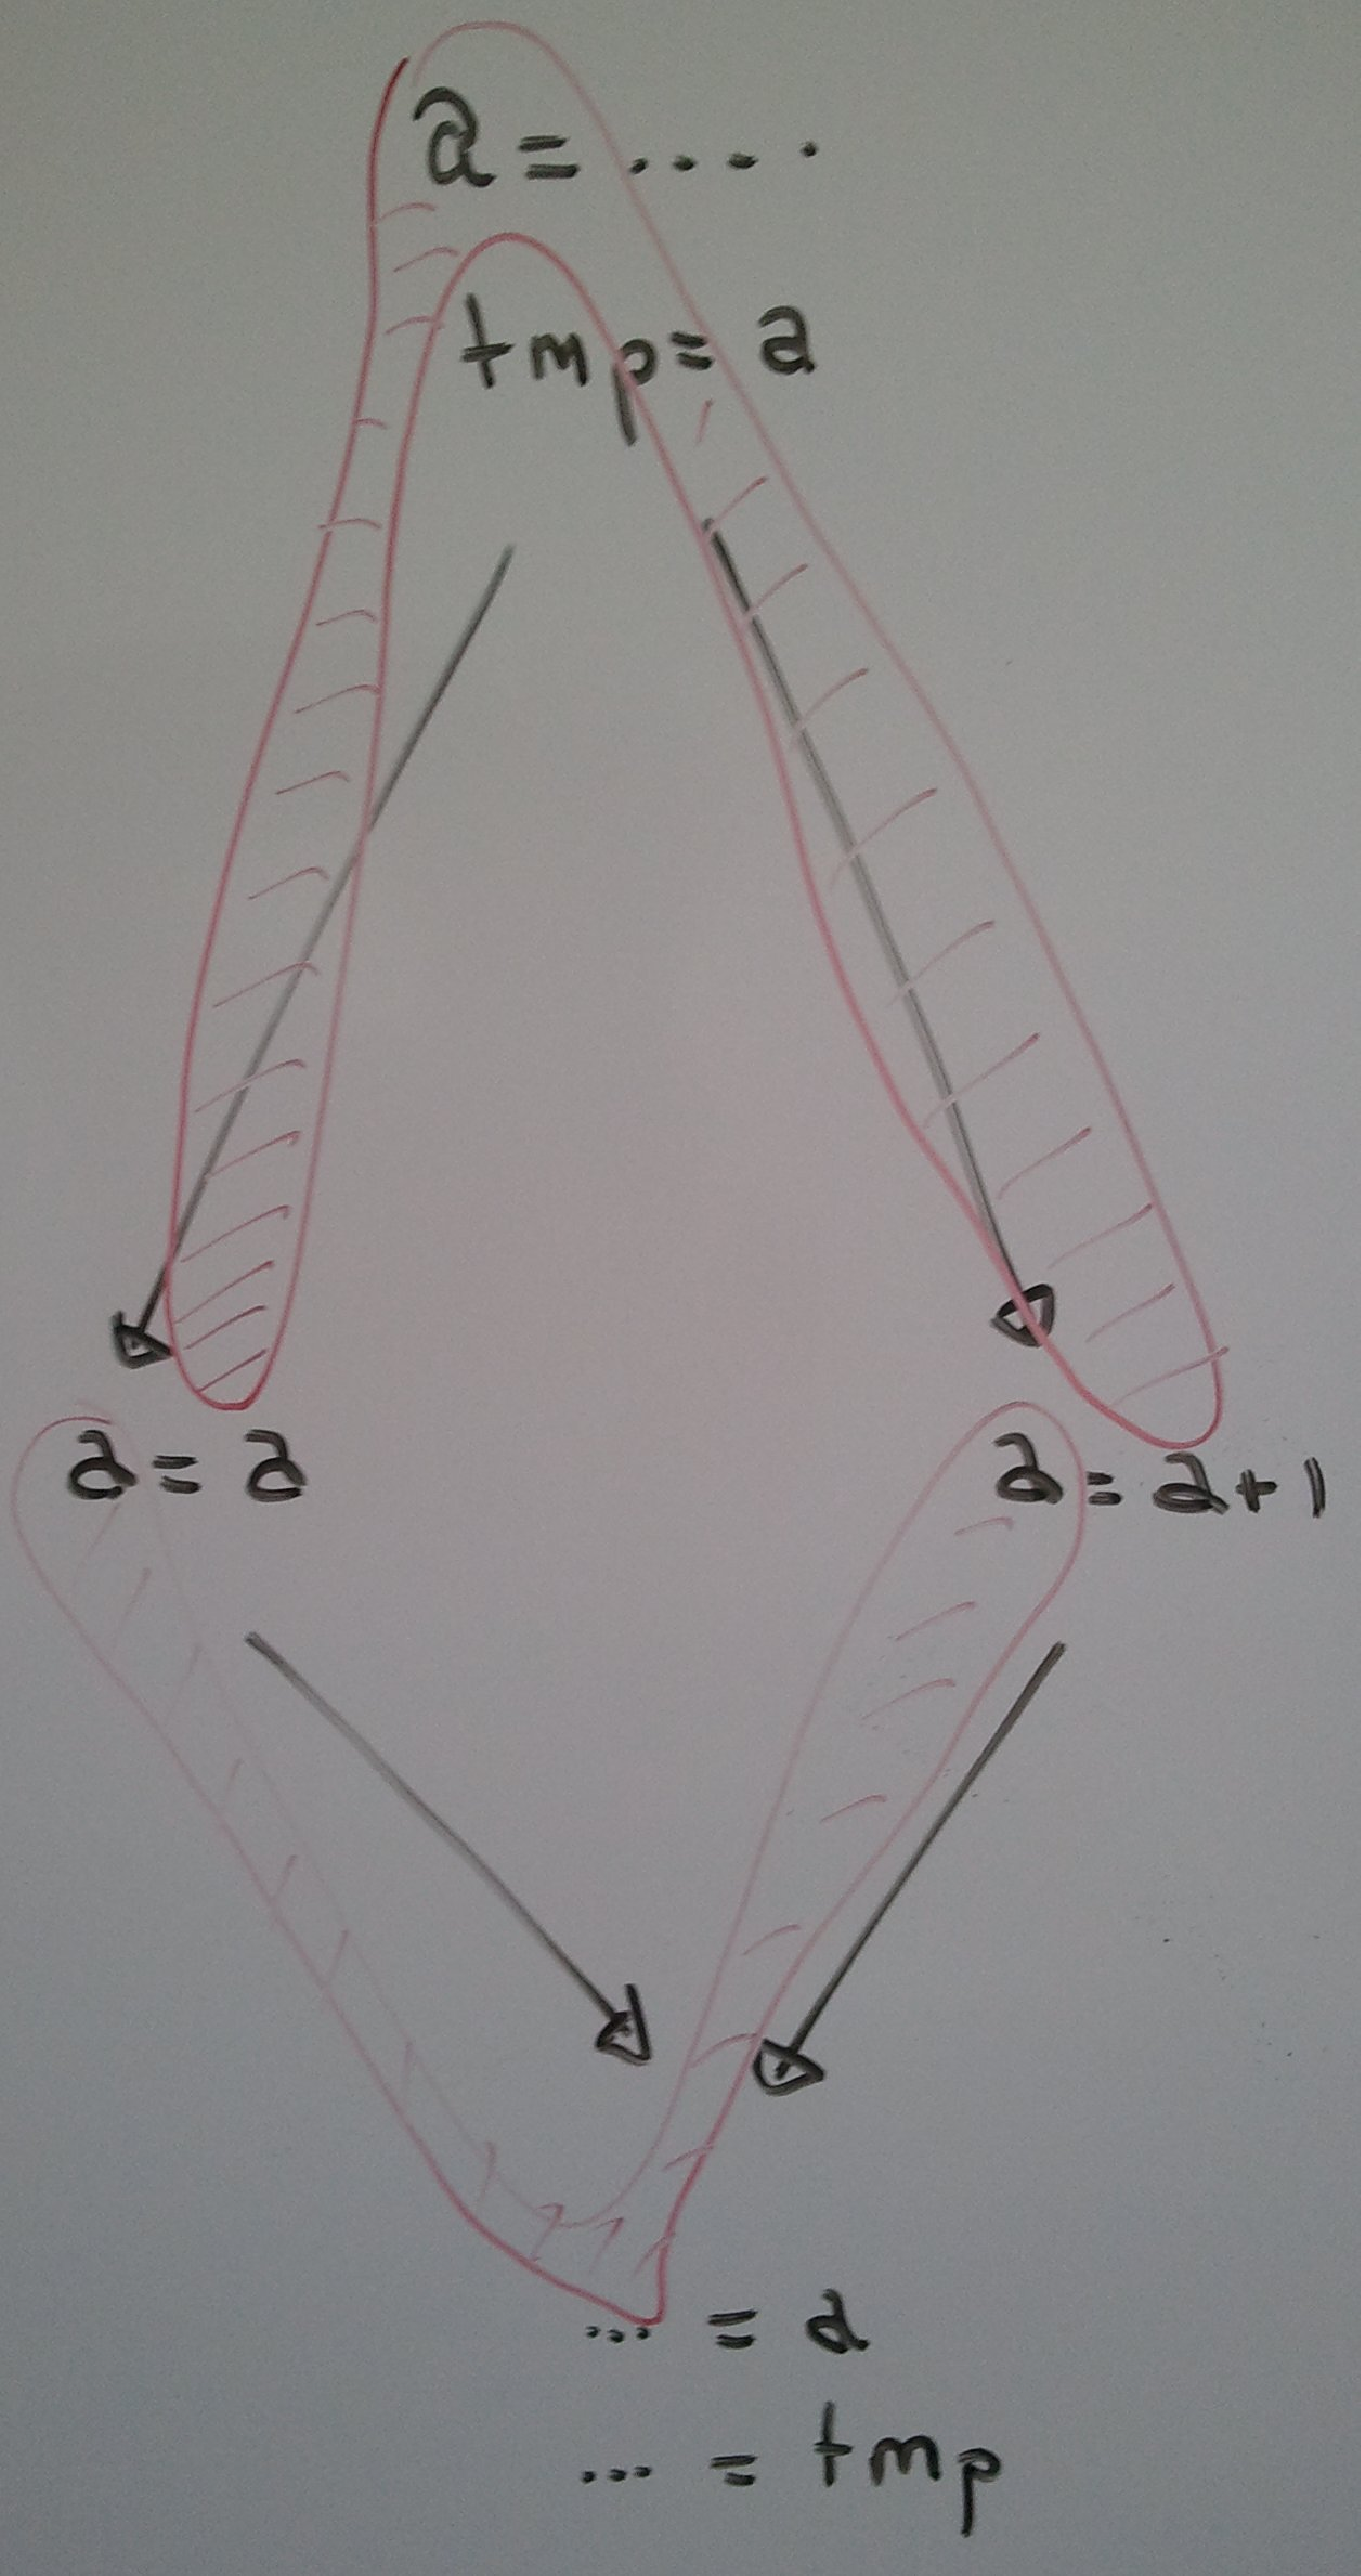
\includegraphics[width=0.3\textwidth]{conventional-a.pdf} &
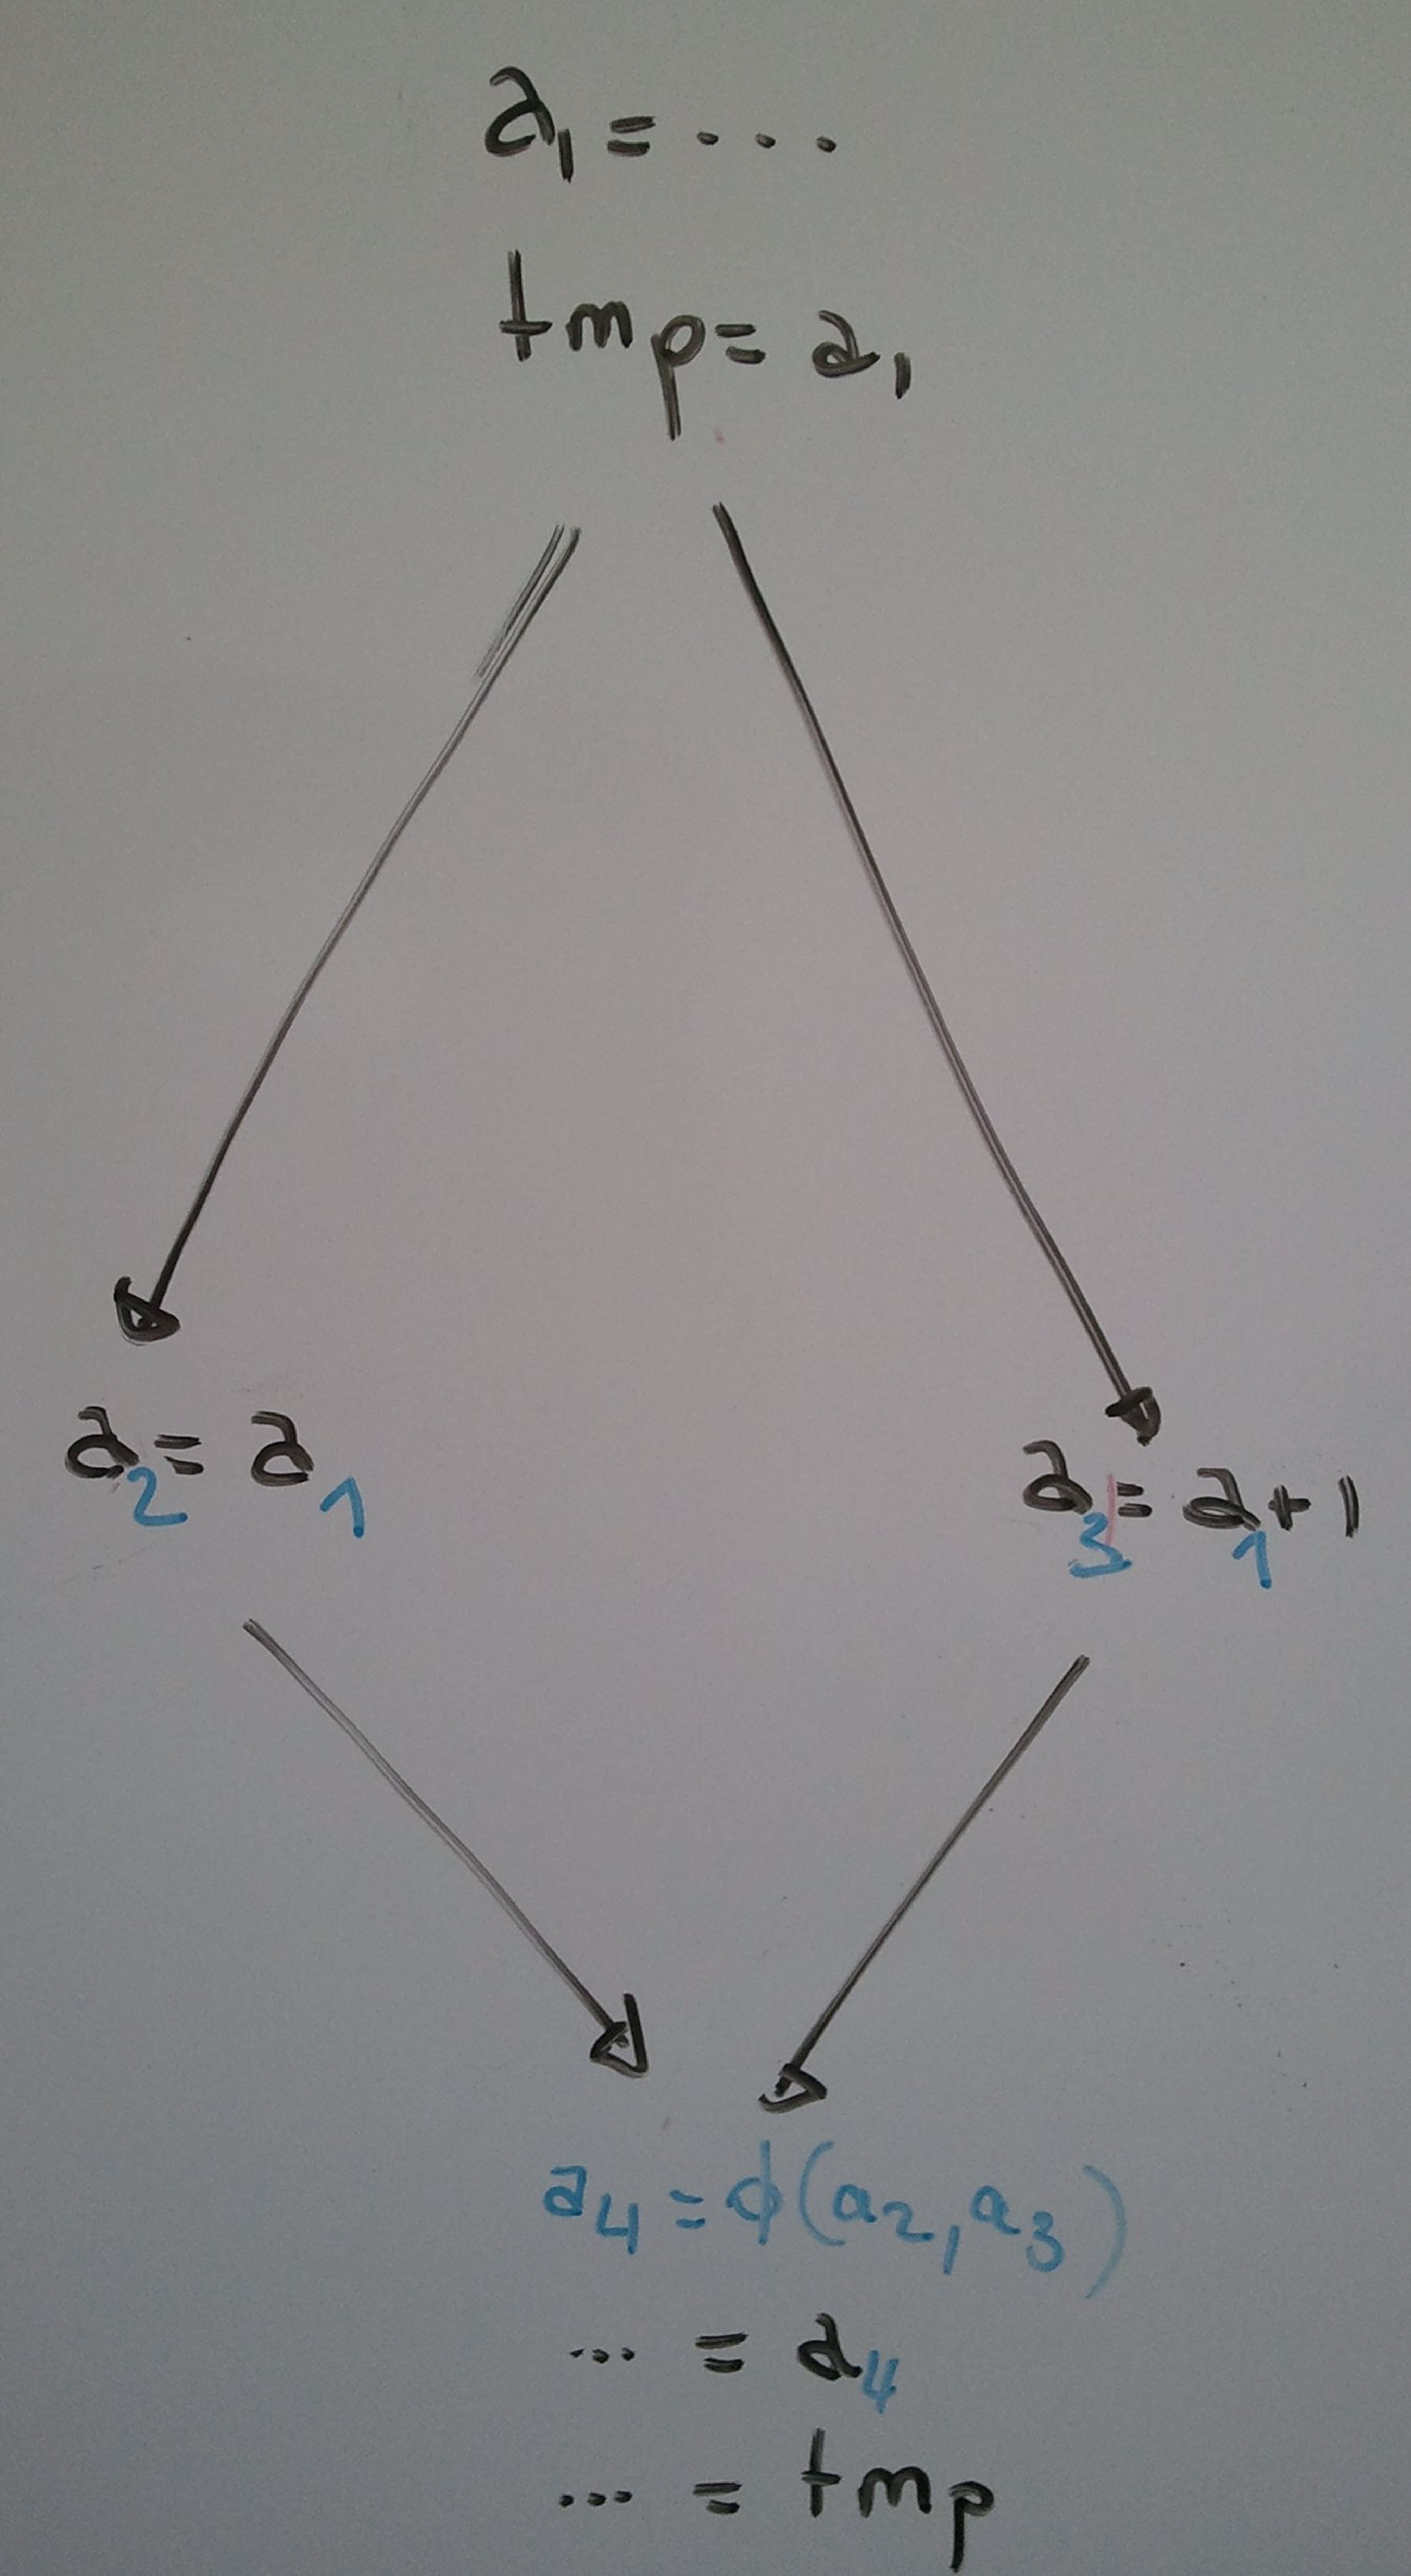
\includegraphics[width=0.3\textwidth]{conventional-b.pdf} &
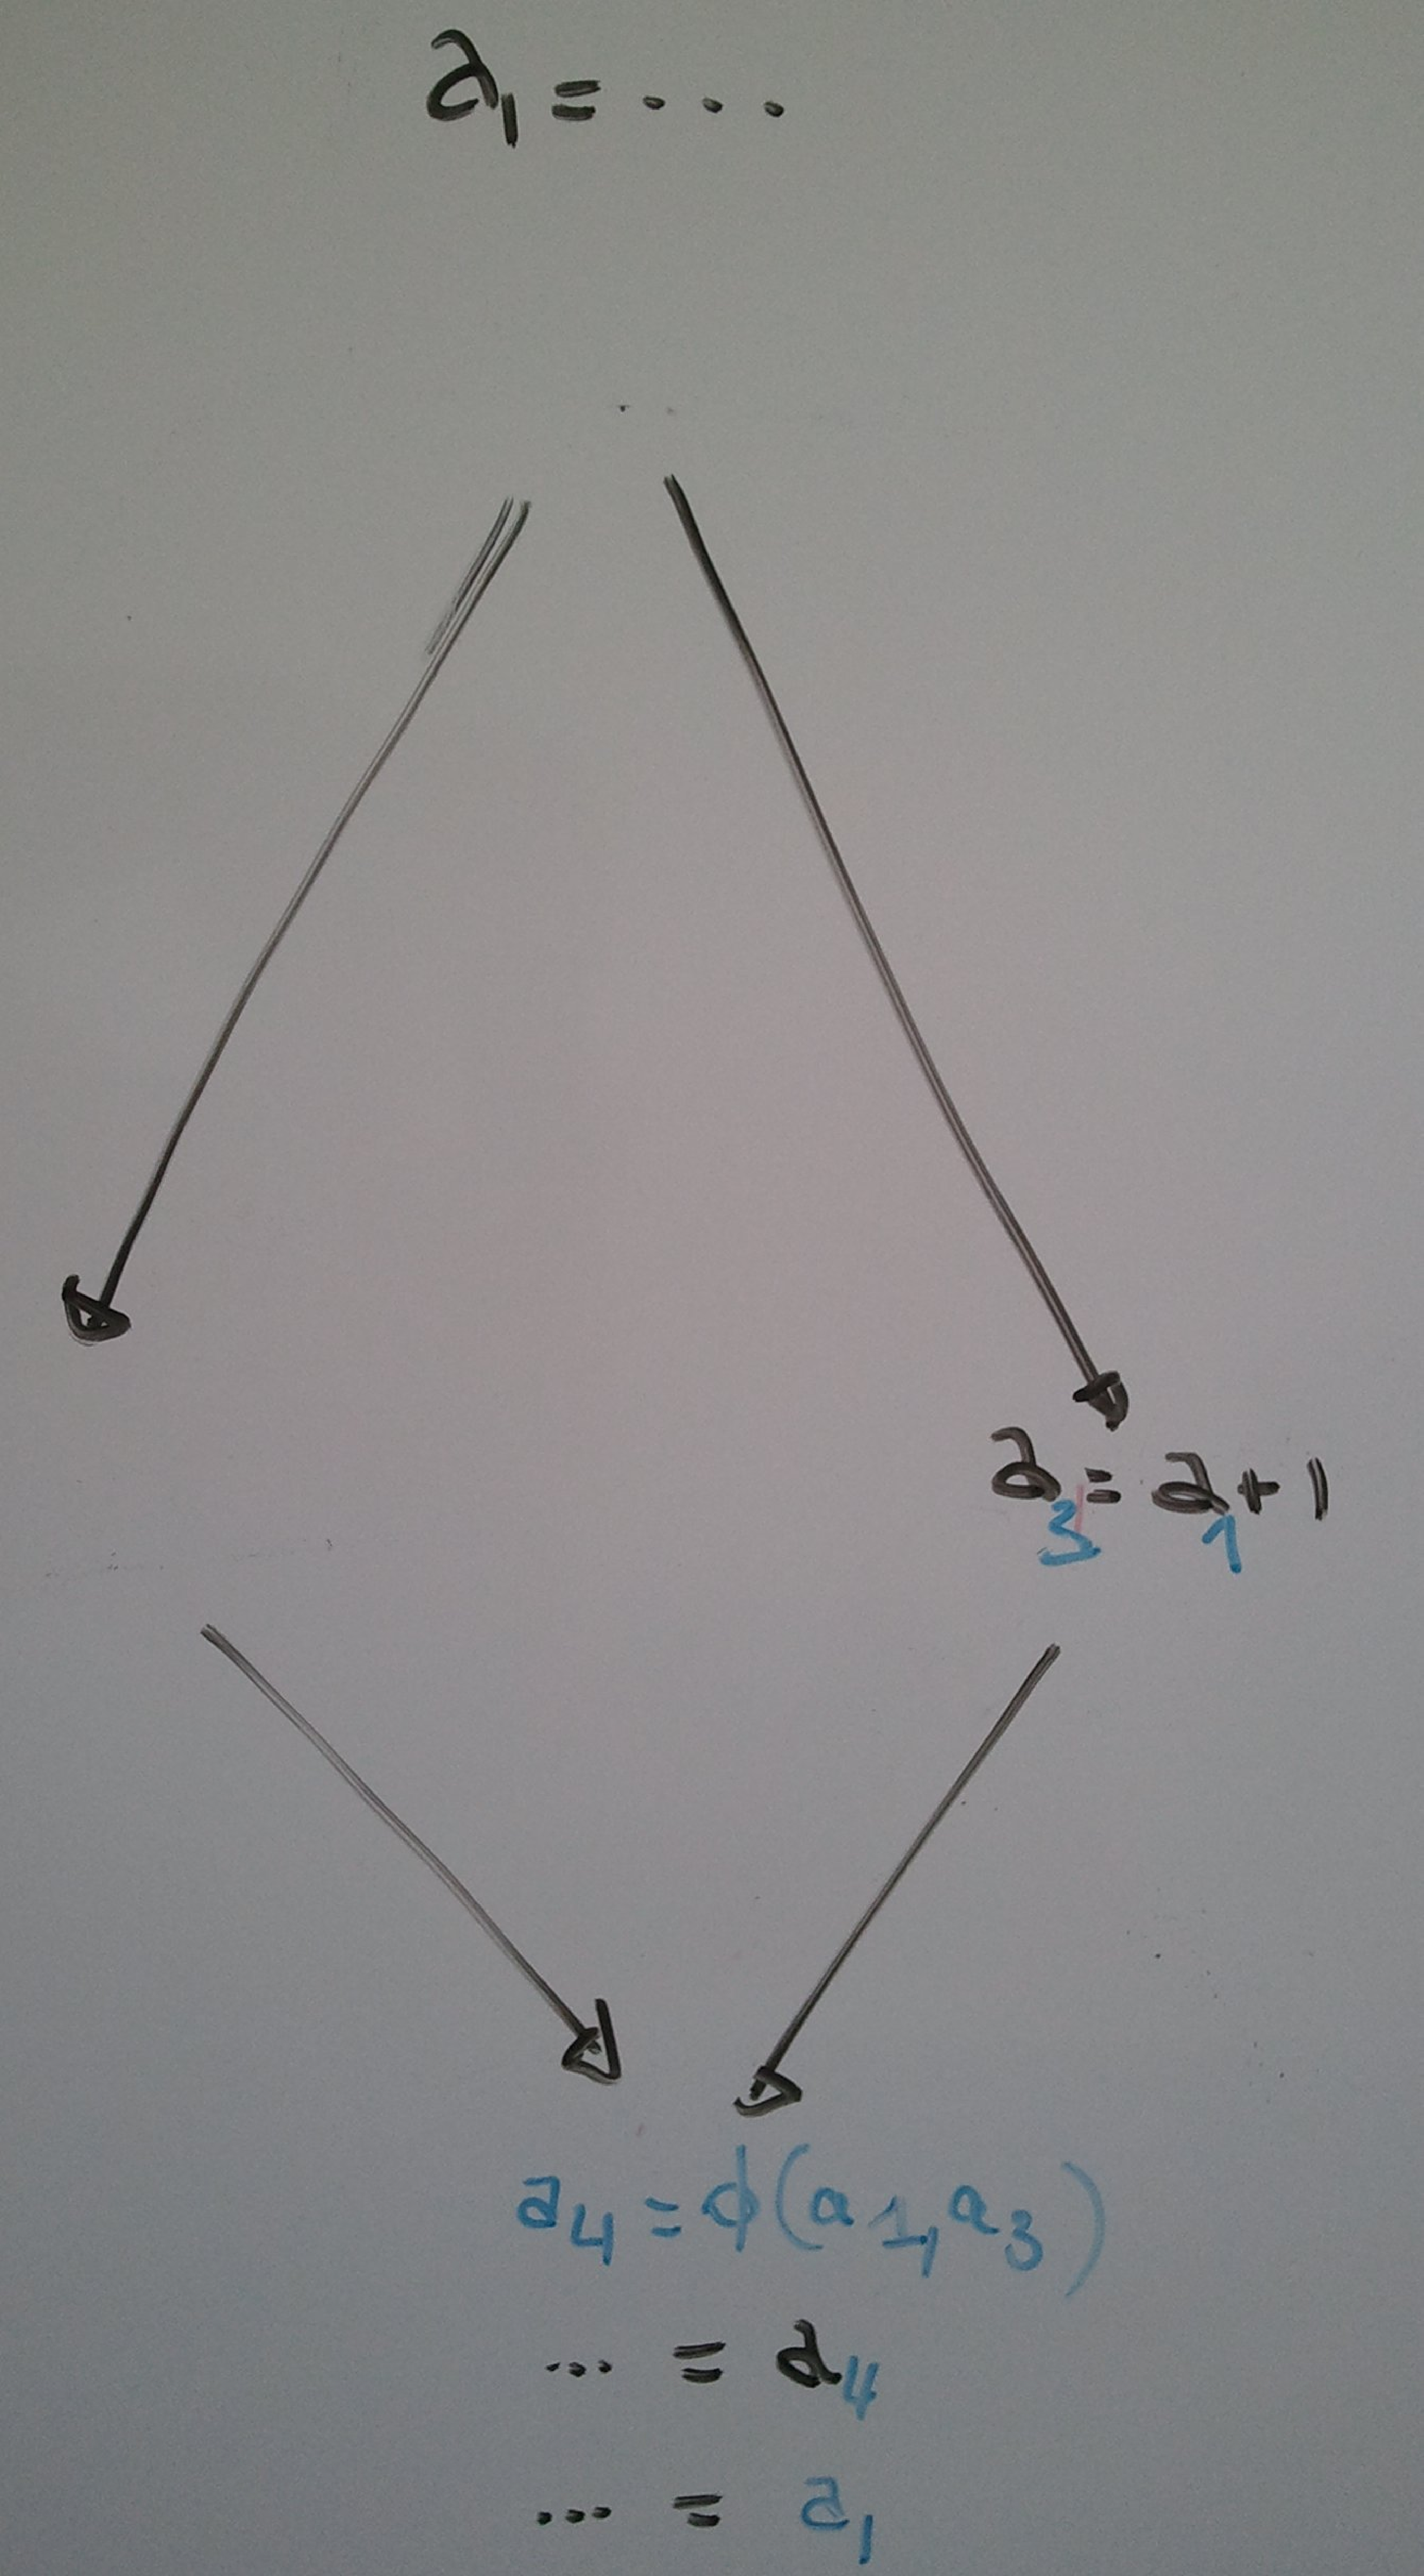
\includegraphics[width=0.3\textwidth]{conventional-c.pdf} \\
(a) the two webs of variable $a$ & 
(b) the two corresponding $\phi$-webs $\{a_1\}$ and $\{a_2,a_3,a_4\}$ &
(c) after propagating $a_1$, SSA form is not conventional anymore
\end{tabular}
\caption{\label{fig:properties_and_flavors:conventional}Non-SSA register webs and corresponding SSA $\phi$-webs; conventional and corresponding transformed SSA form}
\end{figure}



\section{A Stronger Definition of Interference}
\label{sec:properties_and_flavors:ultimate_interference}
Throughout this chapter, two variables have been said to interfere
if their live ranges intersect. Intuitively, two variables with overlapping
lifetimes will require two distinct storage locations; otherwise, a write
to one variable will overwrite the value of the other. In particular,
this definition has applied to the discussion of interference graphs
and the definition of conventional SSA form, as described above.

Although it suffices
for correctness, this is a fairly restrictive definition of interference, based on static considerations. 
The ultimate notion of interference, that is obviously undecidable because of a reduction to the Halting problem, should decide for two distinct variables whether there exists an execution for which they simultaneously hold two different values. 
Several ``static'' extensions to our simple definition are still possible, in which,
under very specific conditions, variables whose live ranges overlap
one another may not interfere. 
We present two examples.

Firstly, consider the double-diamond graph of Figure~\ref{fig:properties_and_flavors:dom_property}(a) again, which although non-strict, is correct as soon as the two if-conditions are the same.
Even if $a$ and $b$ are unique variables with overlapping live
ranges, the paths along which $a$ and $b$ are respectively used and
defined are mutually exclusive with one another. In this case, the
program will either pass through the definition of $a$ and the use
of $a$, or the definition of $b$ and the use of $b$, since all
statements involved are controlled by the same condition, albeit
at different conditional statements in the program. Since only
one of the two paths will ever execute, it suffices to allocate a 
single storage location that can be used for $a$ or $b$. Thus, $a$
and $b$ do not actually interfere with one another. A simple way to refine the interference test is to 
check if one of the variable is live at the definition point of the other. 
This relaxed but correct notion of interference would not make $a$ and $b$ of Figure~\ref{fig:properties_and_flavors:dom_property}(a) interfere while variables $a_1$ and $b_1$ of Figure~\ref{fig:properties_and_flavors:dom_property}(b) would still interfere. This example illustrates the fact that live-range splitting required here to make the code fulfill the dominance property may lead to less accurate analysis results.
As far as the interfere is concerned, for a SSA code with dominance property, the two notions are strictly equivalent: two live-ranges intersect iff one contains the definition of the other.  

Secondly, consider two variables $u$ and $v$, whose live ranges overlap.
If we can prove that $u$ and $v$ will always hold the same value
at every place where both are live, then they do not actually interfere
with one another. Since they always have the same value, a single 
storage location can be allocated for both variables, because there
is only one unique value between them. 
Of course, this new criteria is in general undecidable.
Still, a technique such as global value numbering that is straightforward to implement under SSA (See Chapter~\ref{sec:pre_not_helped:GVN}) can make a fairly good job, especially in the presence of a code with many variable-to-variable copies, such as one obtained after a naive 
SSA destruction pass (See Chapter~\ref{classical_construction_algorithm}).
In that case (See Chapter~\ref{chapter:alternative_ssa_destruction}), the difference between the refined notion of interference and non-value based one is significant. 

This refined notion of interference has significant implications if
applied to SSA form. In particular, the interference graph of a procedure
is no longer chordal, as any edge between two variables whose lifetimes
overlap could be eliminated by this property. 


\section{Further readings}
The advantages of def-use and use-def chains provided for almost free under SSA are well illustrated in chapters~\ref{chapter:constant_propagation_is_easier} and~\ref{chapter:ssi}.

The notion of minimal SSA and a corresponding efficient algorithm to compute it were introduced by Cytron et al. in~\cite{CytronOct91}. For this purpose they extensively develop the notion of dominance frontier of a node $n$, ${\cal DF}(n)=\J(n,r)$. The fact that $\J^+(S)=\J(S)$ have been actually discovered later, and Wolfe gives a simple proof of it in~\cite{WolfeJul94}. More details about the theory on (iterated) dominance frontier can be found in chapters~\ref{chapter:classical_construction_algorithm} and~\ref{alternative_construction_algorithm}. The post-dominance frontier, which is its symmetric notion, also known as the control dependence graph finds many applications. Further discussions on control dependence graph can be found in Chapter~\ref{chapter:vsdg}. 

Most SSA papers implicitly consider the SSA form to fulfill the dominance property. The first technique that really exploits the structural properties of the strictness is the fast SSA destruction algorithm developed by Budimlic et al. in~\cite{BudimlicJun02} and revisited in Chapter~\ref{chapter:alternative_ssa_destruction}. 

The notion of pruned SSA  have been introduced in~\cite{ChoiJan91}. The example of Figure~\ref{fig:properties_and_flavors:pruned} to illustrate the difference between pruned and non pruned SSA have been borrowed from~\cite{CytronOct91}. 
The notions of conventional and transformed SSA were introduced by Sreedhar et al. in their seminal paper~\cite{SreedharSep99} for destructing SSA form.
The description of the existing techniques to turn a general SSA into either a minimal, a pruned, a conventional, or a strict SSA is provided in Chapter~\ref{chapter:classical_construction_algorithm}.

The ultimate notion of interference was first discussed by Chaitin in his seminal paper~\cite{Chaitin81} that presents the graph coloring approach for register allocation. His interference test is similar to the refined test presented in this chapter. In the context of SSA destruction, Chapter~\ref{chapter:alternative_ssa_destruction}, addresses the issue of taking advantage of the dominance property with this refined notion of interference.
 

